%%%%%%%%%
% TO DO %
%%%%%%%%%
% Expand intro
% Redo graphs from graphing program, expand scope, involve 
% More detail
% Actually describe motivation again
% Rewrite into based off previous chapters

\chapter{Approach force curves}

Further to the previous work done in liquid AFM operation, further force curves were taken with a silica-tipped cantilever interacting with a borosilca surface (petri-dish) in a controlled liquid. For each of the curves a controlled concentration of LiCl was added to a 50:50 mix of deionised water and glycerol. Initially the curves were too noisy and unrefined to be taken directly from the machine, thus a script was written and refined over the months from the previous report. For each curve a minimum of 100 curves were binned and averaged into a master curve, with any anomalous lone curves removed. These curves were then analyzed through a python script that corrects the resultant curves from the machine by leveling the noise floor across all curves (\textit{Fig.1}) and defining the contact area linearly (\textit{Fig.2}). 


\newpage

While the initial curves taken on the machine were too noisy, further repeats and refinements to the procedure eventually resulted in 14 averaged curves taken; 7 concentrations with 2 different contact areas taken. Finally these curves were then further tested primarily by analyzing the derivative of the curve and the calculated debye length taken from the exponent of the curve. Additional further dignostic curves were produced and checked by eye for every single curve taken into the average, resulting in well over several thousand total curves processed and checked (\textit{Fig.3}).

\begin{figure}[!tbph]
  \centering
  \subfloat[Site 1 curves.]{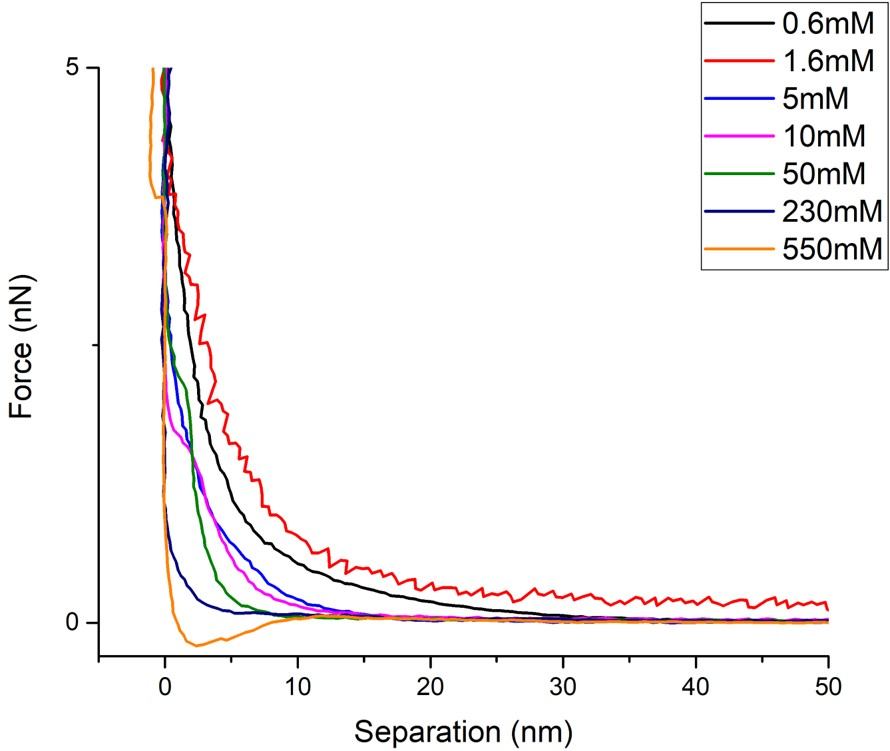
\includegraphics[width=0.45\textwidth]{chapter5/Comparison1.jpg}\label{fig:C1}}
  \hfill
  \subfloat[Site 2 curves.]{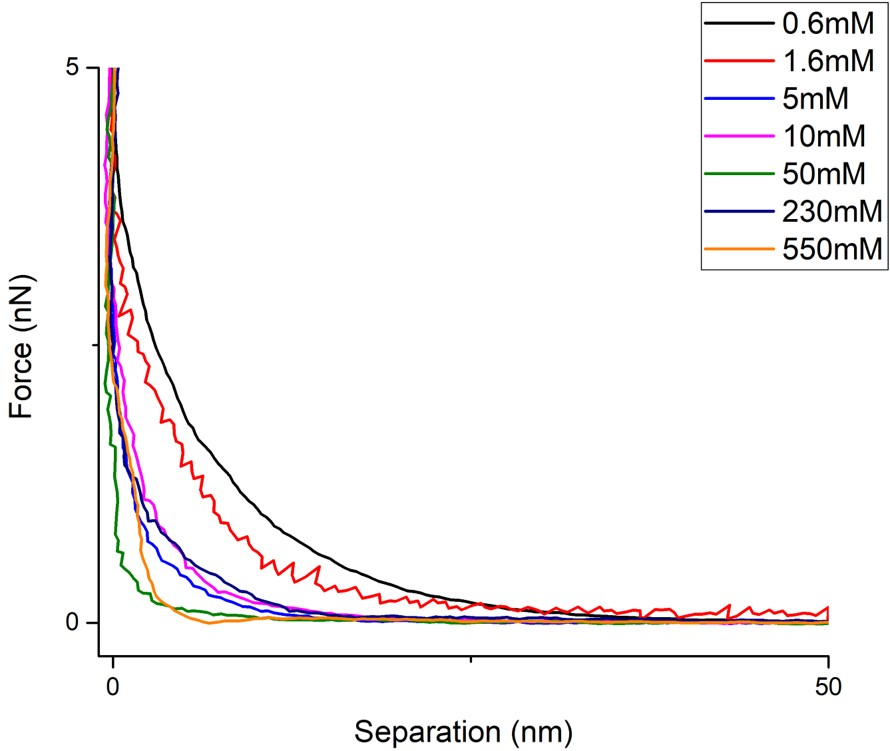
\includegraphics[width=0.45\textwidth]{chapter5/Comparison2.jpg}\label{fig:C2}}
  \caption{The resultant averaged force curves for each of the concentrations. (a) showing the curves taken for the initial contact site and (b) showing the curves taken for the second contact site. }
\end{figure}

Finally the repulsive force was derived from the curves (the repulsive force applied on the cantilever at contact between the tip and the surface) (\textit{Fig.4}). This was done by tuning the fitting parameters of the curves, then analysing the resultant curves over and over until an optimal was found. The contact area parameter were then altered over +/-10nm of the visually derived optimal to calculate the range. If a better fit was found, the optimal was recentered, additionally the range was reduced in the case of a clearly incorrect fit.

\begin{figure}[!tbph!!!]
  \centering
  \subfloat[Site 1 curves.]{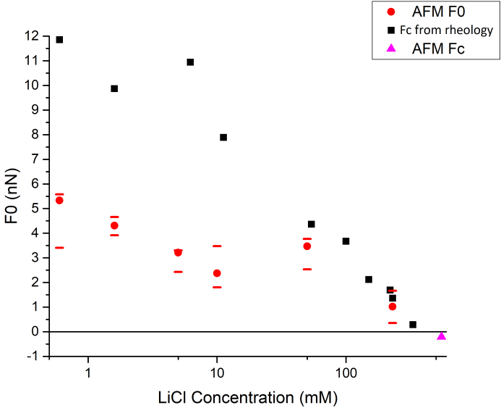
\includegraphics[width=0.45\textwidth]{chapter5/ContF1.png}\label{fig:CF1}}
  \hfill
  \subfloat[Site 2 curves.]{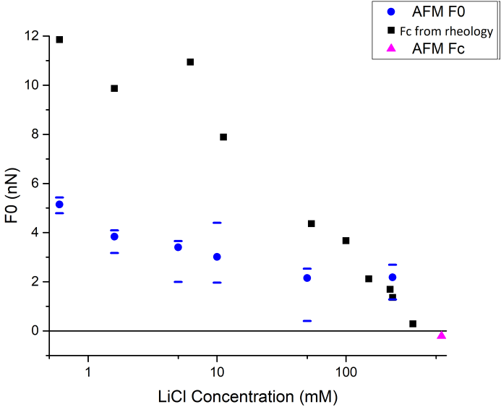
\includegraphics[width=0.45\textwidth]{chapter5/ContF2.png}\label{fig:CF2}}
  \caption{The resultant calculated repulsive force between the surface and the tip. The AFM data is compared against data taken from rheology. In the case of 550mM the repulsive forces transition to attractive, corresponding to the onset stress transitioning into yield stress (as seen from rheological data). F0 is taken from when the curve is within the onset of the contact region, Fc is taken from when the curve bends towards the surface, at the onset of contact (observable in \textit{Fig.3}. (a) and (b) are site 1 and 2 respectively\cite{John}.}
\end{figure}

\newpage

\subsubsection{Analysis of Silica-silica retract curves}

Further analysis is currently being performed on the retract curves utilizing an adapted version of the approach script. This is done in a similar method to the previous, with parameters refined by eye, then the range tested by adding or subtracting 10nm to the contact fitting region. The literature surrounding silica-silica force curves taken in salt usually omit the retract curves, while only a few mention them \cite{Retrace}. 

\cite{John}.


\section{Introduction}

\newpage

\subsection{0.6mM}

\newpage.
\newpage

\subsection{1.6mM}

\newpage.
\newpage

\subsection{5mM}

\newpage.
\newpage

\subsection{10mM}

\newpage

\subsection{25mM}

\newpage

\subsection{50mM}

\newpage

\subsection{230mM}

\newpage.
\newpage

\subsection{550mM}

\newpage.
\newpage

\section{Effects of hydrodynamics}

\newpage.
\newpage

\section{Dwell time effects}

\newpage.
\newpage.
\newpage

\section{pH effects}

\newpage
\newpage

\section{Force mapping}